\documentclass[tikz,border=12pt]{standalone}
\usepackage[T1]{fontenc}
\usepackage{mathpazo}
\usepackage{amsmath,amssymb}
\usetikzlibrary{arrows.meta, positioning, calc, fit, decorations.pathreplacing}

\definecolor{stblue}{HTML}{7B97AD}
\definecolor{rwgold}{HTML}{B8995E}
\definecolor{sage}{HTML}{7A9A7E}
\definecolor{dkbrown}{HTML}{3D3530}
\definecolor{wmgray}{HTML}{7B7067}
\definecolor{cream}{HTML}{F9F6F0}
\definecolor{border}{HTML}{D4C9B8}
\definecolor{terracotta}{HTML}{C47A6A}
\definecolor{lavender}{HTML}{907EA0}

\begin{document}
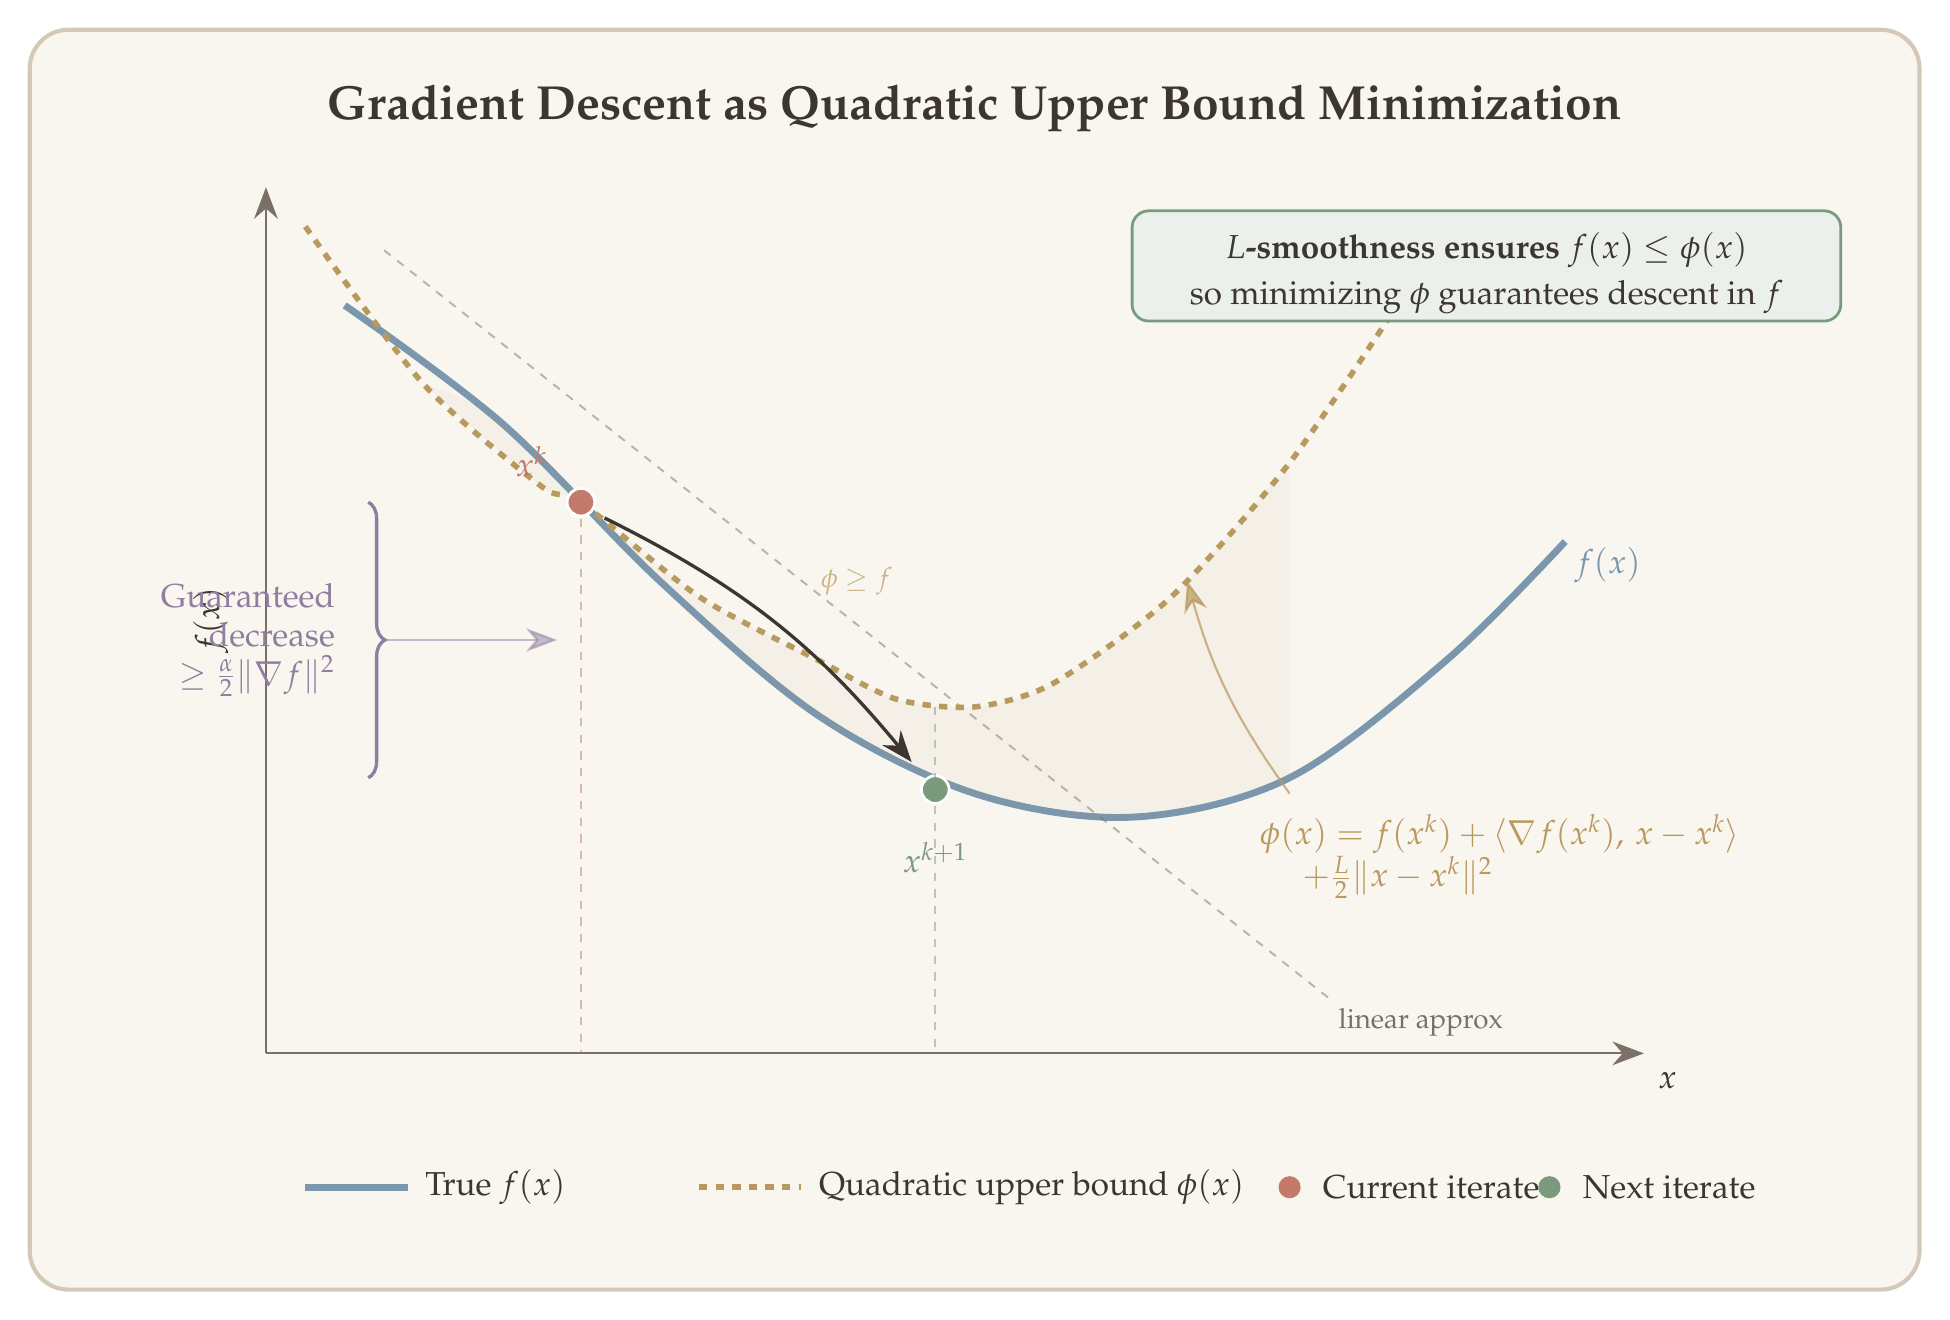
\begin{tikzpicture}[>={Stealth[length=4mm, width=3mm]}]

% Background
\fill[cream, rounded corners=14pt] (-1.5,-1.5) rectangle (22.5,14.5);
\draw[border, line width=1.5pt, rounded corners=14pt] (-1.5,-1.5) rectangle (22.5,14.5);

% Title
\node[text=dkbrown, font=\LARGE\bfseries] at (10.5,13.5) {Gradient Descent as Quadratic Upper Bound Minimization};

% Axes
\draw[wmgray, line width=0.8pt, ->] (1.5,1.5) -- (19.0,1.5);
\draw[wmgray, line width=0.8pt, ->] (1.5,1.5) -- (1.5,12.5);
\node[text=dkbrown, font=\large] at (19.3,1.15) {$x$};
\node[text=dkbrown, font=\large, rotate=90] at (0.8,7.0) {$f(x)$};

% --- True function f(x) ---
% Designed so that the quadratic upper bound at x^k is ALWAYS above f(x)
% f dips from left to a minimum around x=13, then rises
\draw[stblue, line width=2.5pt] plot[smooth, tension=0.55] coordinates {
  (2.5,11.0) (4.5,9.5) (6.5,7.5) (8.5,5.8) (10.5,4.8) (12.5,4.5) (14.5,5.0) (16.5,6.5) (18.0,8.0)};
\node[text=stblue, font=\large\bfseries, right] at (18.0,7.7) {$f(x)$};

% --- Tangent line at x^k (dashed, gray) ---
% x^k is at roughly (5.5, 8.5). Slope ~ -1.3
\draw[wmgray, line width=0.7pt, dashed, opacity=0.5] (3.0,11.7) -- (15.0,2.2);
\node[text=wmgray, font=\normalsize, right] at (15.0,1.9) {linear approx};

% --- Quadratic upper bound phi(x) ---
% Tangent to f at x^k=(5.5, 8.5), parabola opening upward
% The parabola MUST be above f everywhere visible
% phi(x) = 8.5 - 1.3*(x-5.5) + 0.16*(x-5.5)^2  (approximately)
% Minimum at x_min = 5.5 + 1.3/(2*0.16) = 5.5 + 4.06 = 9.56, phi_min ~ 5.85
\draw[rwgold, line width=2pt, dashed] plot[smooth, tension=0.45] coordinates {
  (2.0,12.0) (3.5,10.0) (5.0,8.7) (5.5,8.5) (7.0,7.3) (8.5,6.5) (9.5,6.0)
  (10.5,5.9) (11.5,6.2) (13.0,7.3) (14.5,9.0) (16.0,11.2)};

% Light shading between phi and f to show "phi >= f"
\fill[rwgold, opacity=0.06] plot[smooth, tension=0.45] coordinates {
  (3.5,10.0) (5.0,8.7) (5.5,8.5) (7.0,7.3) (8.5,6.5) (9.5,6.0)
  (10.5,5.9) (11.5,6.2) (13.0,7.3) (14.5,9.0)}
  -- plot[smooth, tension=0.55] coordinates {
  (14.5,5.0) (12.5,4.5) (10.5,4.8) (8.5,5.8) (6.5,7.5) (4.5,9.5) (3.5,10.0)}
  -- cycle;

% --- Current point x^k ---
\fill[terracotta] (5.5,8.5) circle (5pt);
\draw[white, line width=1pt] (5.5,8.5) circle (5pt);
\node[text=terracotta, font=\large\bfseries, above left] at (5.2,8.7) {$x^k$};

% --- Next point x^{k+1} = minimizer of phi ---
% phi minimum at ~ (10.0, 5.9)
% f at x=10.0 is about 4.9
\fill[sage] (10.0,4.85) circle (5pt);
\draw[white, line width=1pt] (10.0,4.85) circle (5pt);
\node[text=sage, font=\large\bfseries, below] at (10.0,4.3) {$x^{k+1}$};

% Arrow showing the GD step
\draw[dkbrown, line width=1.2pt, ->] (5.8,8.3) to[bend left=12] (9.7,5.2);

% Dashed vertical at x^{k+1} showing gap between phi and f
\draw[sage, line width=0.7pt, dashed, opacity=0.5] (10.0,5.9) -- (10.0,4.85);
\draw[terracotta, line width=0.7pt, dashed, opacity=0.5] (5.5,8.5) -- (5.5,1.5);
\draw[sage, line width=0.7pt, dashed, opacity=0.5] (10.0,4.85) -- (10.0,1.5);

% --- Guaranteed decrease bracket ---
\draw[lavender, line width=1.2pt, decorate, decoration={brace, amplitude=6pt, mirror}]
  (2.8,5.0) -- (2.8,8.5);
\node[text=lavender, font=\large, left, align=right] at (2.5,6.75)
  {Guaranteed\\ decrease\\ $\geq \frac{\alpha}{2}\|\nabla f\|^2$};
% Leader arrow
\draw[lavender, line width=0.8pt, ->, opacity=0.5] (3.0,6.75) -- (5.2,6.75);

% --- Upper bound formula label ---
\node[text=rwgold, font=\large, right, align=left] at (14.0,4.0)
  {$\phi(x) = f(x^k) + \langle \nabla f(x^k),\, x - x^k \rangle$\\
   $\quad\; + \tfrac{L}{2}\|x - x^k\|^2$};
\draw[rwgold, line width=0.8pt, ->, opacity=0.7] (14.5,4.8) to[bend left=10] (13.2,7.5);

% --- Key property box ---
\fill[sage!15, rounded corners=6pt] (12.5,10.8) rectangle (21.5,12.2);
\draw[sage, line width=1pt, rounded corners=6pt] (12.5,10.8) rectangle (21.5,12.2);
\node[text=dkbrown, font=\large\bfseries] at (17.0,11.7)
  {$L$-smoothness ensures $f(x) \leq \phi(x)$};
\node[text=dkbrown, font=\large] at (17.0,11.1)
  {so minimizing $\phi$ guarantees descent in $f$};

% --- phi >= f annotation ---
\node[text=rwgold, font=\normalsize\itshape, opacity=0.7] at (9.0,7.5) {$\phi \geq f$};

% Legend
\draw[stblue, line width=2.5pt] (2.0,-0.2) -- (3.3,-0.2);
\node[text=dkbrown, font=\large, right] at (3.4,-0.2) {True $f(x)$};
\draw[rwgold, line width=2pt, dashed] (7.0,-0.2) -- (8.3,-0.2);
\node[text=dkbrown, font=\large, right] at (8.4,-0.2) {Quadratic upper bound $\phi(x)$};
\fill[terracotta] (14.5,-0.2) circle (4pt);
\node[text=dkbrown, font=\large, right] at (14.8,-0.2) {Current iterate};
\fill[sage] (17.8,-0.2) circle (4pt);
\node[text=dkbrown, font=\large, right] at (18.1,-0.2) {Next iterate};

\end{tikzpicture}
\end{document}
